\documentclass[]{article}
\usepackage{lmodern}
\usepackage{float}
\usepackage[margin=1in]{geometry}
\usepackage{amssymb,amsmath}
\usepackage{ifxetex,ifluatex}
\usepackage{fixltx2e} % provides \textsubscript
\ifnum 0\ifxetex 1\fi\ifluatex 1\fi=0 % if pdftex
  \usepackage[T1]{fontenc}
  \usepackage[utf8]{inputenc}
\else % if luatex or xelatex
  \ifxetex
    \usepackage{mathspec}
  \else
    \usepackage{fontspec}
  \fi
  \defaultfontfeatures{Ligatures=TeX,Scale=MatchLowercase}
\fi
% use upquote if available, for straight quotes in verbatim environments
\IfFileExists{upquote.sty}{\usepackage{upquote}}{}
% use microtype if available
\IfFileExists{microtype.sty}{%
\usepackage{microtype}
\UseMicrotypeSet[protrusion]{basicmath} % disable protrusion for tt fonts
}{}
\usepackage{hyperref}
\hypersetup{unicode=true,
            pdfborder={0 0 0},
            breaklinks=true}
\urlstyle{same}  % don't use monospace font for urls
\usepackage{graphicx,grffile}
\makeatletter
\def\maxwidth{\ifdim\Gin@nat@width>\linewidth\linewidth\else\Gin@nat@width\fi}
\def\maxheight{\ifdim\Gin@nat@height>\textheight\textheight\else\Gin@nat@height\fi}
\makeatother
% Scale images if necessary, so that they will not overflow the page
% margins by default, and it is still possible to overwrite the defaults
% using explicit options in \includegraphics[width, height, ...]{}
\setkeys{Gin}{width=\maxwidth,height=\maxheight,keepaspectratio}
\IfFileExists{parskip.sty}{%
\usepackage{parskip}
}{% else
\setlength{\parindent}{0pt}
\setlength{\parskip}{6pt plus 2pt minus 1pt}
}
\setlength{\emergencystretch}{3em}  % prevent overfull lines
\providecommand{\tightlist}{%
  \setlength{\itemsep}{0pt}\setlength{\parskip}{0pt}}
\setcounter{secnumdepth}{0}
% Redefines (sub)paragraphs to behave more like sections
\ifx\paragraph\undefined\else
\let\oldparagraph\paragraph
\renewcommand{\paragraph}[1]{\oldparagraph{#1}\mbox{}}
\fi
\ifx\subparagraph\undefined\else
\let\oldsubparagraph\subparagraph
\renewcommand{\subparagraph}[1]{\oldsubparagraph{#1}\mbox{}}
\fi

\date{}

\begin{document}

\section{HemeWeb: Container based high performance computing scenario in
cloud infrastructure for
HemeLB}\label{hemeweb-container-based-high-performance-computing-scenario-in-cloud-infrastructure-for-hemelb}

\subsection{Steven Steven - s1561690}\label{steven-steven---s1561690}

\subsection{I. Introduction}\label{i.-introduction}

HemeLB is a fluid dynamics simulation software package that is developed
for the study of blood flow {[}1{]}. Researches in computational biology
have used HemeLB to help with their study. Some of its latest use are
simulating blood vessel development in mouse {[}2{]} and its retina
{[}3{]}. Another study used HemeLB to study vascular blood flow
abnormalities in human eye {[}4{]}. The software package works by
constructing a 3D model of blood vessels, and then approximating the
equation governing fluid flow within. This allows scientists and doctors
to estimate how blood will flow in the given vessels. It is evident that
HemeLB simulation is important for medical study. Furthermore, HemeLB is
envisioned to be an integral part of future medical decisions {[}5{]}.

However, it is currently complex to configure and run the software
packages. The complete workflow comprises of many steps that need many
tools to run. Scientists and doctors might not have the capabilities to
configure these tools. Furthermore, the resources needed to run these
workflow also varies widely depending on the case. While small cases can
run on a laptop, scientifically interesting cases require parallel
computing resources, like the ARCHER supercomputer, to run. In addition,
for each step of the workflow, different interfaces are required; from
command line to graphical user interface. These factors limits HemeLB's
user to few individuals currently.

Furthermore, the HemeLB project needs to improve the trustworthiness of
its simulation. This trust, on top of HemeLB being usable, is important
to make it a part of any medical decision. Simulation results should be
easy to audit and easy to reproduce. These characteristics allow peers
to review the simulation and confirm the result. Currently, there are
some measures in HemeLB for reproduction and audit. Its source code is
available for public on GitHub, making it possible to audit the
software. Furthermore, the system includes some tools to automatically
record version used, and the input parameters. These steps allow peers
to build the software and replicate a simulation, albeit in a manual
way. With recent pushes for open science and reproducible computing
research {[}6, 7, 8{]}, an extra step for being open is justified.

To address these problems, I propose to create an extension to HemeLB
called HemeWeb. HemeWeb will be a web application that will hide the
complexity of configuration from its users. Also, it will allow
automatic recording of simulations, making it easy to examine and
reproduce simulations. I will use cloud infrastructure and
containerization technology to help address the issues outlined. In
brief, this project will make HemeLB simulations usable and more open.

\subsection{II. Background}\label{ii.-background}

To develop the extension with proper functions, I need to elaborate some
information. These are about the current HemeLB workflow, the
infrastructures, containerization technology, and how similar project
tackle similar problems.

\textbf{Current HemeLB Workflow}

Figure 1 illustrates the current steps in the HemeLB workflow. I will
now ellaborate on each steps.

\begin{figure}[H]
\centering
\includegraphics{../resources/images/HemeLB-workflow.png}
\caption{Overview of current HemeLB workflow}
\end{figure}

\begin{enumerate}
\def\labelenumi{\arabic{enumi}.}
\tightlist
\item
  \textbf{Geometrical model reconstruction}
\end{enumerate}

Before preparing a simulation, users require a 3D model of the vessels
they wish to simulate. This step is out of the scope of this project but
typically involves taking a 2D image of blood vessels or 3D CT scan data
and constructing its 3D representation in a .stl format. This step
typically run in a workstation with problem-dependant tools and
interface.

\begin{enumerate}
\def\labelenumi{\arabic{enumi}.}
\setcounter{enumi}{1}
\tightlist
\item
  \textbf{Domain definition}
\end{enumerate}

In this step, users' inputs about simulation parameters are needed. User
needs to configure simulation parameters like blood viscosity, inlet and
outlet placements, and other conditions. A graphical user interface has
been developed for this purpose. Allowing doctors and users to use it
easily on a workstation without resorting to command line interface.
These information are then encoded into a profile file that will be used
in the next step.

\begin{enumerate}
\def\labelenumi{\arabic{enumi}.}
\setcounter{enumi}{2}
\tightlist
\item
  \textbf{Geometry generation}
\end{enumerate}

In this step, the 3D model of blood vessel's surface and the simulation
parameters are combined to produce a description of the 3D domain,
i.e.~a list of every point in space to be simulated and its properties,
and the other simulation parameters. This step can be time consuming as
it is currently not parallel, but can run on a workstation.

\begin{enumerate}
\def\labelenumi{\arabic{enumi}.}
\setcounter{enumi}{3}
\tightlist
\item
  \textbf{HemeLB simulation}
\end{enumerate}

This step is where the bulk of the computations are done. The
information encoded from previous steps is given as input to the main
HemeLB application. It is an efficiently MPI-parallel SPMD program that
can efficiently use from 1 up to 32,000 cores {[}9{]}. Typical problems
use around 500 cores. Very simple problems can be run on a workstation,
while demanding cases will require an HPC infrastructure. Users need to
use command line interface to do this step.

\begin{enumerate}
\def\labelenumi{\arabic{enumi}.}
\setcounter{enumi}{4}
\tightlist
\item
  \textbf{Post processing}
\end{enumerate}

Simulation results from previous steps are encoded in a format that is
efficient to wwrite in parallel but is not easily viewed. To view the
simulation in a graphical way, further processing is needed. This is
where post-processing steps will do its work. This step will convert the
files into a VTK format, a de facto standard in computational science,
that can be viewed with many tools such as Paraview {[}10{]} and VisIt
{[}11{]}. This process run on workstation with a command line interface.

\textbf{HPC Infrastructure and HemeLB}

Computational biology and bioinformatics often use mathematical and
computation approaches in their research. They use these approaches to
help answer questions and understand experiments in biology {[}9{]}.
While small cases can run on a laptop, more complex case demand parallel
computing resources like ARCHER supercomputer. HemeLB is a prime example
of computational biology software that need these better computing
resources. Its most demanding part, HemeLB simulation, currently run on
ARCHER supercomputer {[}1{]}.

Traditionally, there are two paradigm that tackles large computing
processes. These are High Performance Computing and High Throughput
Computing (HTC). HPC involve using many similar computing nodes to
perform tightly coupled computations. These nodes are often placed in
the same room and connected with high bandwidth network. These network
allow the nodes to communicate between each other in doing the
computations {[}10{]}. An example for this type of resources are
computer clusters, GPUs, and supercomputers. In contrast, HTC allow
heterogeneous computing resources to cooperate for common goals. These
resources are often distributed geographically and varies in type and
performance. These resources will then do different independent
computations that independently scheduled {[}10{]}. Based on these
distinctions, HPC is a correct categorization of HemeLB.

However, running these simulations requires access to HPC
infrastructures that might not have reproducibility of a research as a
priority. Facilities that operate these infrastructure often give out
computing hour usage to projects based on the merit of their
peer-reviewed proposal, for example how PRACE {[}11{]}, the Partnership
for Advanced Computing in Europe, and EPSRC {[}12{]} give access to
their infrastructure to researchers. This means that those seeking to
reproduce computation of a research have to compete with other projects
for the limited computing hours that are given out by these
institutions. Most likely, it will not be the top priority, hence
creating barrier for reproducing computational research.

Not being prioritized in these facilities create a barrier for HemeLB to
become more trustworthy because reproduction of simulation is
non-trivial. As iterated on the previous section, HemeLB project have
taken the steps to address reproducibility of the simulation by manually
recording all the configurationns, tools version, input files,
parameters and result of the simulation. Anyone theoritically could
request these documentation and reproduce the result with the
appropriate computing resource. However, research facility that will
prioritize more important research inherently will limit people that
want to reproduce the computation result significantly. This is where
cloud computing infrastructure enter the picture.

\textbf{Cloud Computing}

In response to the huge demand for computational power by researchers
and academics, a concept called grid computing was envisioned in 1990s
{[}13{]}{[}14{]}. This vision considered computing resources analogous
to power grid, where user should not care from where the resources are
acquired and how it is delivered to the user. This paradigm was mainly
developed with the interest of researchers and academia that the
business models caters to the most {[}15{]}. Grid computing typically
give CPU hours based on the proposal that is vetted by the institutions.
Example of this institution is TeraGrid which operates until 2011
{[}16{]}.

Cloud computing shares similar vision with the grid computing paradigm,
in that the computing resources are acquired and delivered are invisible
to the users, but different on the execution of the business model. It
is massively scalable, allows abstract encapsulation of computing
resources, dynamicaly configured and delivered on-demand and most
importantly, driven by economies of scale {[}15{]}. Since it is driven
by economies of scale, it is in the interest of cloud providers to
provide features that users actually need and want to pay for, therefore
creating a tight feedback loop between users and the providers to
develop the platform better than how grid computing handle feature
developments.

This has allowed cloud vendors to grow significantly, for example in
2013 it was noted that some cloud vendors could reach more than 90\%
growth per annum {[}17{]}. This growth further fuels demand and allow
them to cut pricing for their service multiple times
{[}18{]}{[}19{]}{[}20{]} and create more demands. This development has
allowed businesses and institutions to offload their computational need
to the cloud vendors for a price rather than building their own
infrastructure. This scenario could also be used for our purpose of
performing or reproducing computational research without needing to have
access to large HPC systems.

Cloud vendors like Amazon also capitalize on the need for computing
resources for HPC applications {[}10{]}. Running HPC applications on
cloud platforms, while incurring performance overhead, can be a viable
alternative to supercomputers as shown by the nekkloud project {[}21{]},
NASA HPC Applications {[}22{]}, and HPC applications benchmark in cloud
case study {[}23{]}. Also, part of this project is to demonstrate that
HemeLB can run acceptably on a cloud platform.

\textbf{How other HPC projects deal with similar problems}

In the past few years, many complex HPC software packages have been
deployed to the cloud. In this section, I will highlight these projects
to learn how they solve similar issues.

One similar project is Nekkloud {[}21{]}. In this case, Nektar++, a
complex high-order finite element code, face similar usability problems.
Their original workflow was so complex that only few people can run it.
People without computer expertise had a hard time to actually run
computations with it. Furthermore, one should also get access to a HPC
infrastructure to run it, which may not be easy. Nekkloud project is
their answer to these problems. It was developed to encapsulate most
difficulties in using the software package. Using a web application to
provide high level interface instead of using the command line. Making
it more accessible to more people without computing expertise. In
addition to that, it ran on cloud infrastructures. Allowing people
without dedicated HPC infrastructure to run high-order finite element
computations.

Another project that is tackling similar space is Galaxy {[}24{]}.
Galaxy, a web-based reproducible research platform, uses cloud
infrastructure to run its HPC applications. In illustrating its use, the
developers have developed a super-resolution spark (SRS) model. This
modeling process needs a supercomputing resources to execute the cloud
infrastructure provides. These capabilities are also encapsulated in an
easy to use web interfaces, making it easy for scientists to run, and
share simulations.

Above examples illustrate that a web application can be a viable
alternative interface for complex applications. However, this
implementation on the cloud also has a negative impact on the
applications. Raw performance is lower than dedicated HPC
infrastructures. These performance penalty was observed in the projects
mentioned already {[}21{]}{[}23{]}{[}24{]}. Nekkloud authors considered
the performance penalty acceptable, because the cloud infrastructures
allow flexibility. This flexibility and the benefit of making it more
usable will sometimes outweigh the performance penalty.

Pros and cons of web application for complex HPC projects are area that
are often discussed. But, deployment scenario for these HPC projects in
cloud infrastructure are rarely discussed. More specifically, the use of
containerization technology in helping tools deployment.

One of the above projects, Galaxy, support containerization technology
for their tools packaging. They used docker, one implementation of linux
container software. Galaxy claimed that using docker allow efficiency,
isolation, and portability of their tools {[}25{]}. These are good
traits that could also be helpful for HemeLB. However, their main
contribution to the literature is not on this usage. They focus more on
how Galaxy can support reproducible research. Usage of containerization
technology are sparsely detailed.

Containerization technology are often benchmarked in high performance
computing area. These researches {[}26{]}{[}27{]} have tried to discuss
using container technology in HPC space. Also, shifter project {[}28{]}
try to unleash docker on HPC infrastructure. Meaning, allowing their HPC
infrastructure to use docker capabilities. Yet, none have discussed the
effect of containerization in running HPC application in cloud. This is
where I envision this project could contribute on. Adding more details
to the effect of containerization technology on cloud based HPC
applications. Docker, in particular, are often discussed as a promising
technology to support reproducible research {[}29{]}. Complex HPC
application like HemeLB is a prime example where this is a problem.
Especially, when there are many push for open science {[}6, 7, 8{]} and
easy reproduction.

\subsection{III. Main Claim}\label{iii.-main-claim}

In this project, I will show that the proposed approach will help the
HemeLB project by improving the workflow's usability, auditability, and
reproducibility. In this section, I will define what I mean by these
terms and outline how I will measure success.

Also, to support these claims, I will develop an experimental web
application called HemeWeb. HemeWeb will use container technology to run
HemeLB simulations on cloud infrastructure. It will be the basis of
future deployment in other commodity hardware infrastructure. For
instance, Hospitals would want patient-related simulations to run on
their own infrastructures.

\begin{itemize}
\tightlist
\item
  \textbf{Usability}
\end{itemize}

I will define usability in this project as the ease of use of the
software to run a simulation. HemeWeb will reduce cognitive efforts
needed to run said simulations. Enabling non computer expert, defined as
people who never compile a C program, to run blood flow simulation with
simple documentation. I will measure this usability criteria along four
metrics of usability that Nielsen {[}32{]} use. These metrics are
success rate, time needed, error rate, and user's satisfaction on
running a simulation.

\begin{itemize}
\tightlist
\item
  \textbf{Reproducibility}
\end{itemize}

Ease of reproducing a simulation is the definition of reproducibility in
this project. Users, given enough information, should be able to
reproduce past simulations with ease. HemeWeb will provide
reproducibility by enabling user to reproduce past simulations with
simple interface. On top of that, the web application will make it easy
to run a simulation with past parameters. Enabling easy reproduction of
past simulations. Like how I measure usability criteria, I will also
measure reproducibility along four metrics. These are success rate, time
needed, error rate, and user's satisfaction on reproducing a past
simulation.

\begin{itemize}
\tightlist
\item
  \textbf{Auditability}
\end{itemize}

I will define auditability as the ease of other parties to confirm and
audit a simulation. HemeWeb will record and publish tools,
configurations, input files, and simulation results. The use of
containerization technology will help capture and publish these
information. Especially, when the containerization technology publish
the image on a public registry. This in the end, will encourage
peer-review which will further improve trust. The same four metrics as
above criteria will be used to measure this.

In measuring these 3 criteria, I will run a usability testing at the
evaluation period. I will use direct observation, with semi-structured
interview technique to capture the desired metrics. More details will be
provided in the methodology section.

\subsection{IV. Methods}\label{iv.-methods}

In developing the web application, I need to compare the available
technologies. One instance where this choice is important is the choice
of containerization technology. Whichever tools I choose, will have to
adhere to the criteria set on previous section. Those criteria are
improving usability, reproducibility, and auditability. In addition to
that, I will add few other criteria to select the appropriate tools.
These could be developer familiarity, features available, and ease of
usage of the tools. Based on these combined criteria, I will then select
the final implementation to be used on the project. To make sure that
this choices is appropriate, I have been and will continue to read about
the subject. Also, I will discuss the proposed method with my peers and
supervisors.

Next, I have to make sure that the methods chosen in measuring success
is appropriate. For this, I will follow DECIDE framework outlined in
this book {[}30{]}. In the previous section, each criteria can be
measured by 4 metrics. They are success rate, time needed, error rate,
and user's satisfaction on doing tasks. Users testing at the evaluation
period will be used to measure these metrics. I will ask users to do two
task; to run and reproduce a simulation using both old and new approach.
Running a simulation will capture usability metrics for both approach.
While reproducing a simulation will capture metrics for both
reproducibility and auditability.

I will then observe users doing their tasks. From these observations, I
can capture the first three metrics. Are they giving up? How long does
it take to run a simulation using one of the approach? How many times do
they ask for help? Did they find out that the past simulation result is
faulty? These are the kind of questions that I will capture from the
observation. For the last metrics, satisfaction, I will use a
semi-structured interview. This is important to first ask their
satisfaction level in an objective, numerical, way. And then continue
with qualitative questions to probe more about their experience. These
questions are going to be designed in the evaluation preparation period.

However, this usability test will have some limitations. First, these
tests will take considerable amount of time, roughly 30 minutes per
respondent. To run a simulation, one should go through few steps. And in
the test, a user will run four simulation in total. Two for each task,
comparing both approaches. Consequently, this increase of cognitive
burden may influence the test results to some extends. To minimize this
risk, I have to make sure that the tasks are one of the simplest one.
Making it less demanding for the users to run a task. However, running
these tasks will still need considerable duration. Second limitation is
the limited number of users involved in the tests. With the long
required durations, the number of tests to be done will be limited. On
top of that, it will be a challenge to ask a lot of doctors and
scientists to do the tests. The limited number of test results will only
allow the analysis to be an indicative measure of how HemeWeb improve
usability, reproducibility, and auditability.

\subsection{V. Implementation}\label{v.-implementation}

This section will elaborate the work plan and risks for the project. The
project period starts from 2nd of June 2016 to 19th August 2016. In this
period, I will work on 4 major tasks. They are the project preparation,
execution, evaluation and dissertation writing. Each of these tasks can
overlap with each other because of the limited time and many tasks to
do. For example, project execution and evaluation will overlap from
middle of July. This is intentional because these tasks can run in
parallel. With this plan, I have determined that the scope of this
project is doable in the duration given. Especially when I structure the
project to allow graceful degradation.

\begin{figure}[H]
\centering
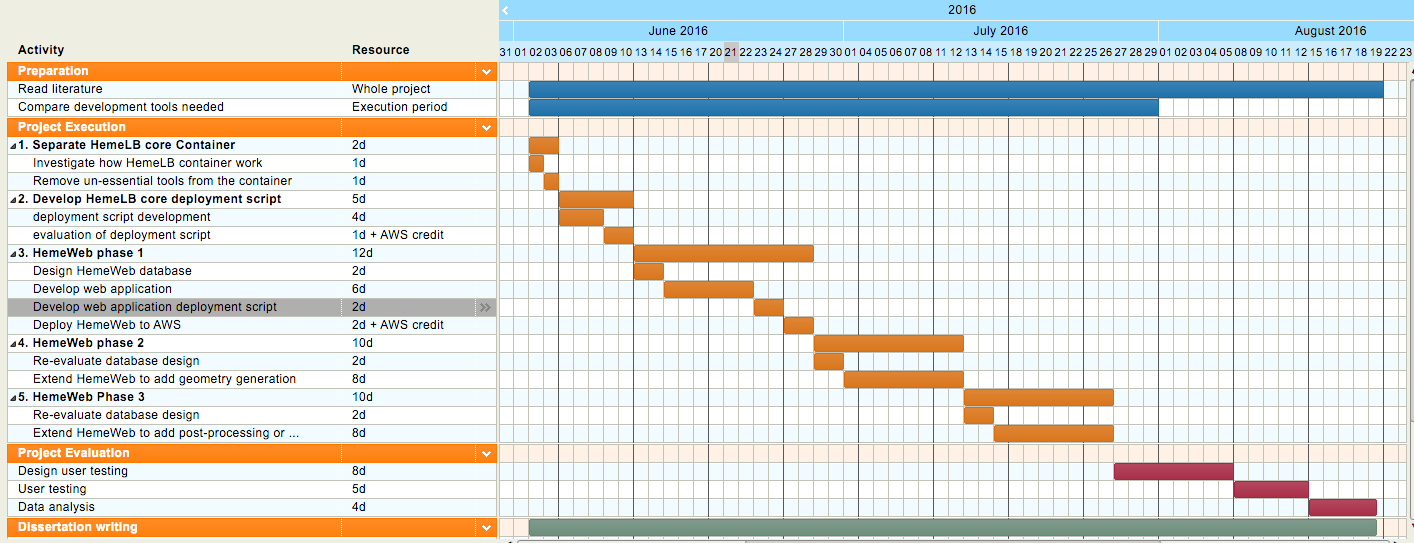
\includegraphics{../resources/images/workplan.png}
\caption{Project Work Plan}
\end{figure}

\begin{itemize}
\tightlist
\item
  \textbf{HemeWeb development plan}
\end{itemize}

HemeWeb will be a web application that hides the complexity of running
HemeLB simulations. Web application will enable users to interface with
a HemeLB simulation via internet browser. Internet browser is such a
standard tools that many people can use. Allowing doctors and scientists
to run simulation without worry of configurations and complexity.

Besides being a web application, HemeWeb will also use containerization
technology. Allowing the web app to tie down simulation result with the
tools used. Having this automatic record will enable easy reproduction
and easy audit for interested parties. Furthermore, using container
technology will allow HemeWeb to swap tools. Currently, to run
simulation with different version of the tools, one should reconfigure
everything. Container technology will allow HemeWeb to swap the tools
easily. Allowing users to run simulation with different version of tools
without worrying about configurations.

In a nutshell, HemeWeb will replace part of HemeLB simulation workflow
like illustrated in figure 3. The first phase of the development will
make sure one of the steps to run simulation can run in the cloud. With
more and more integrations, more part of the workflow will run in the
cloud. This will pave ways for making the simulation workflow run
entirely on the browser. Making it even easier for users to run
simulation.

\begin{figure}[H]
\centering
\includegraphics{../resources/images/HemeWeb-scope.png}
\caption{HemeWeb scope}
\end{figure}

In the following section, I will outline how the development of HemeWeb
will go. I have divided the development into 5 separate distinct steps.
They are:

\begin{enumerate}
\def\labelenumi{\arabic{enumi}.}
\item
  \textbf{Separating HemeLB core into its own container}

  Currently, users need to compile HemeLB and other tools on their own
  computer before using it. These configurations are complex and need
  simplification. Hence, developer of HemeLB created a container image
  with complete tools inside,
  https://github.com/mobernabeu/docker-hemelb. However, for HemeWeb,
  this is not ideal. HemeWeb should use a cluster of HemeLB instances to
  run the simulation. These cluster should just contain HemeLB core
  instead of having the full tools available. This is why, separating
  this HemeLB core into its own container should be my first step for
  this project. I will take the currently available image as a basis,
  and remove all the unnecessary tools. HemeLB binary should be the only
  concern of the image.
\item
  \textbf{Orchestrate HemeLB cluster deployment}

  Next, I plan to create a deployment script for HemeLB. I have select
  preliminary tools for deploying the HemeLB image into a cluster.
  However, further investigation in the project execution will be
  necessary. These tools will configure the cluster in an automatic
  fashion so that it is ready for use. I will be able to configure the
  cluster with a script at the end of this task.
\item
  \textbf{Develop HemeWeb to do HemeLB simulation {[}Phase 1{]}}

  This is the first step that HemeWeb will be able to run HemeLB
  simulations. I will develop the prototype web interface that enable
  user to run simulation. User can upload their input files, wait for
  the simulation to finish, and download the result. In this step, I
  will have developed a working prototype. This prototype have the
  smallest scope possible, but still allow simulations to run. The
  system should look like the image below.

  \begin{figure}[H]
  \centering
  \includegraphics{../resources/images/HemeWeb-phase-1.png}
  \caption{Phase 1 of HemeWeb}
  \end{figure}
\item
  \textbf{Extends HemeWeb to handle geometry generation step {[}Phase
  2{]}}

  After finishing with the previous step, I will extend HemeWeb to
  handle more functions. This function is the geometry generation step.
  This step will not result in a different interface for the users, but
  it will expects different input. After this step is complete, HemeWeb
  will now work with extra functionalities. The system should look like
  the image below.

  \begin{figure}[H]
  \centering
  \includegraphics{../resources/images/HemeWeb-phase-2.png}
  \caption{Phase 2 HemeWeb}
  \end{figure}
\item
  \textbf{Extends HemeWeb to handle domain definition step or
  post-processing step {[}Phase 3{]}}

  At this point, there are two possible extensions available for
  HemeWeb. They are the domain definition step or post-processing step.
  Both of these steps need different technical expertise to complete the
  integration. I will decide on the project execution on which function
  I should tackle. This decision will depend on the difficulty, and
  remaining time for the project. However, it has to emphasized that
  even without this step, HemeWeb can still work just fine.
\end{enumerate}

\begin{itemize}
\tightlist
\item
  \textbf{Risks}
\end{itemize}

As with all projects with limited time and budget, there are risks
involved in this project. First is the chance of project execution not
running as planned. This is why, I structure this project to allow it to
gracefully degrade. Meaning that the project will always have a working
product at each checkpoints. This is to make sure that I always having
working prototype at each iteration of the software. Preventing the
chance of having nothing to show at the end of the project. Second, is
the fact that I have to rely on external parties for evaluation. Part of
the evaluation of the proposed system will consists of sending out
questionnaires. I have to make sure that respondents complete the
questionnaires on time. Thus, I structured the evaluation and the
development part to run concurrently. Making sure I give enough time for
respondents and for me to remind them.

\subsection{VI. Output}\label{vi.-output}

This project will create two outputs that HemeLB project will use. They
are:

\begin{enumerate}
\def\labelenumi{\arabic{enumi}.}
\item
  Working HemeWeb prototype

  I will develop the prototype in three phases, divided based on the
  functionalities. In each phase, the prototype will work as a
  standalone application just fine. With each iteration, I will add more
  functions to the prototype. The next section, work plan, will add more
  details on how I will develop the prototype.
\item
  HemeWeb usability guideline

  In the future, HemeWeb can be the interface for doctors to run
  simulations. This means that HemeWeb will need further improvement to
  be ready for general use. Future development can use the work done in
  this project as a basis for usability feature. Thus, I will create a
  usability document derived from the analysis done in this project.
\end{enumerate}

\subsection{References}\label{references}

{[}1{]} Itani, M. A., Schiller, U. D., Schmieschek, S., Hetherington,
J., Bernabeu, M. O., Chandrashekar, H., \ldots{} \& Groen, D. (2015). An
automated multiscale ensemble simulation approach for vascular blood
flow. Journal of Computational Science, 9, 150-155.

{[}2{]} Franco, C. A., Jones, M. L., Bernabeu, M. O., Vion, A. C.,
Barbacena, P., Fan, J., \ldots{} \& Coveney, P. V. (2016). Non-canonical
Wnt signalling modulates the endothelial shear stress flow sensor in
vascular remodelling. Elife, 5, e07727.

{[}3{]} Franco, C. A., Jones, M. L., Bernabeu, M. O., Geudens, I.,
Mathivet, T., Rosa, A., \ldots{} \& Phng, L. K. (2015). Dynamic
endothelial cell rearrangements drive developmental vessel regression.
PLoS Biol, 13(4), e1002125.

{[}4{]} Bernabeu, M. O., Lu, Y., Lammer, J., Aiello, L. P., Coveney, P.
V., \& Sun, J. K. (2015, August). Characterization of parafoveal
hemodynamics associated with diabetic retinopathy with adaptive optics
scanning laser ophthalmoscopy and computational fluid dynamics. In
Engineering in Medicine and Biology Society (EMBC), 2015 37th Annual
International Conference of the IEEE (pp.~8070-8073). IEEE.

{[}5{]} Green, C. (2014, June 14). Computer simulation could become
`integral' in the diagnosis, treatment, or prevention of disease by the
end of the century \textbar{} Science \textbar{} News \textbar{} The
Independent. Retrieved April 4, 2016, from
http://www.independent.co.uk/news/science/computer-simulation-could-become-integral-in-the-diagnosis-treatment-or-prevention-of-disease-by-the-9537730.html

{[}6{]} Donoho, D. L. (2010). An invitation to reproducible
computational research. Biostatistics, 11(3), 385-388.

{[}7{]} Sandve, G. K., Nekrutenko, A., Taylor, J., \& Hovig, E. (2013).
Ten simple rules for reproducible computational research. PLoS Comput
Biol, 9(10), e1003285.

{[}8{]} Peng, R. D. (2011). Reproducible research in computational
science. Science (New York, Ny), 334(6060), 1226.

{[}9{]} Groen, D., Hetherington, J., Carver, H. B., Nash, R. W.,
Bernabeu, M. O., \& Coveney, P. V. (2013). Analysing and modelling the
performance of the HemeLB lattice-Boltzmann simulation environment.
Journal of Computational Science, 4(5), 412-422.

{[}10{]} ParaView homepage. (n.d.). Retrieved April 14, 2016, from
http://www.paraview.org/

{[}11{]} VisIt homepage. (n.d.). Retrieved April 14, 2016, from
https://wci.llnl.gov/simulation/computer-codes/visit/

{[}10{]} Huerta, M., Downing, G., Haseltine, F., Seto, B., \& Liu, Y.
(2000). NIH working definition of bioinformatics and computational
biology. US National Institute of Health.

{[}11{]} Whitepaper: An Introduction to High Performance Computing on
AWS. (2015, August). Retrieved April 4, 2016, from
https://d0.awsstatic.com/whitepapers/Intro\_to\_HPC\_on\_AWS.pdf

{[}12{]} PRACE Research Infrastructure. (n.d.). Retrieved April 4, 2016,
from http://www.prace-project.eu/

{[}13{]} ARCHER » Getting Access to ARCHER. (n.d.). Retrieved April 4,
2016, from http://www.archer.ac.uk/access/

{[}14{]} Berman, Fran, Geoffrey Fox, and Anthony JG Hey. Grid computing:
making the global infrastructure a reality. Vol. 2. John Wiley and sons,
2003.

{[}15{]} Foster, I., \& Kesselman, C. (Eds.). (2003). The Grid 2:
Blueprint for a new computing infrastructure. Elsevier.

{[}16{]} Foster, I., Zhao, Y., Raicu, I., \& Lu, S. (2008, November).
Cloud computing and grid computing 360-degree compared. In Grid
Computing Environments Workshop, 2008. GCE'08 (pp.~1-10). Ieee.

{[}17{]} Extreme Science and Engineering Discovery Environment. (n.d.).
XSEDE \textbar{} TeraGrid Archives. Retrieved April 4, 2016, from
https://www.xsede.org/tg-archives

{[}18{]} FSN \textasciitilde{} Outsourcing \textasciitilde{} The economy
is flat so why are financials Cloud vendors growing at more than 90
percent per annum?. (2013, March 5). Retrieved April 4, 2016, from
http://www.fsn.co.uk/channel\_outsourcing/the\_economy\_is\_flat\_so\_why\_are\_financials\_cloud\_vendors\_growing\_at\_more\_than\_90\_percent\_per\_annum\#.UbmtsPlJPGA/

{[}19{]} Barr, J. (2014, March 26). AWS Price Reduction \#42 -- EC2, S3,
RDS, ElastiCache, and Elastic MapReduce \textbar{} AWS Blog. Retrieved
April 4, 2016, from
https://aws.amazon.com/blogs/aws/aws-price-reduction-42-ec2-s3-rds-elasticache-and-elastic-mapreduce/

{[}20{]} Martin, S. (2014, January 24). Announcing Reduced Pricing on
Storage \textbar{} Blog \textbar{} Microsoft Azure. Retrieved April 4,
2016, from https://azure.microsoft.com/en-us/blog/storage-price-match/

{[}21{]} Lardinois, F. (2014, March 25). Google Announces Massive Price
Drops For Its Cloud Computing Services And Storage, Introduces
Sustained-Use Discounts. Retrieved April 4, 2016, from
http://techcrunch.com/2014/03/25/google-drops-prices-for-compute-and-app-engine-by-over-30-cloud-storage-by-68-introduces-sustained-use-discounts/

{[}22{]} Cohen, Johanne, et al. ``Nekkloud: A software environment for
high-order finite element analysis on clusters and clouds.'' Cluster
Computing (CLUSTER), 2013 IEEE International Conference on. IEEE, 2013.

{[}23{]} Mehrotra, Piyush, et al. ``Performance evaluation of Amazon EC2
for NASA HPC applications.'' Proceedings of the 3rd workshop on
Scientific Cloud Computing Date. ACM, 2012.

{[}24{]} He, Qiming, et al. ``Case study for running HPC applications in
public clouds.'' Proceedings of the 19th ACM International Symposium on
High Performance Distributed Computing. ACM, 2010.

{[}25{]} Walker, M. A., Madduri, R., Rodriguez, A., Greenstein, J. L.,
\& Winslow, R. L. (2016). Models and Simulations as a Service: Exploring
the Use of Galaxy for Delivering Computational Models. Biophysical
journal, 110(5), 1038-1043.

{[}26{]} Moreews, F., Sallou, O., \& Bras, Y. L. (2015, July). A curated
Domain centric shared Docker registry linked to the Galaxy toolshed. In
Galaxy Community Conference 2015.

{[}27{]} Higgins, J., Holmes, V., \& Venters, C. (2015, July).
Orchestrating Docker Containers in the HPC Environment. In High
Performance Computing (pp.~506-513). Springer International Publishing.

{[}28{]} Yu, H. E., \& Huang, W. (2015). Building a Virtual HPC Cluster
with Auto Scaling by the Docker. arXiv preprint arXiv:1509.08231.

{[}29{]} Jacobsen, D. M., \& Canon, R. S. Contain This, Unleashing
Docker for HPC.

{[}30{]} Boettiger, C. (2015). An introduction to Docker for
reproducible research. ACM SIGOPS Operating Systems Review, 49(1),
71-79.

{[}31{]} Sharp, H., Jenny, P., \& Rogers, Y. (2007). Interaction
design:: beyond human-computer interaction.

{[}32{]} Bernabeu, M. O. (n.d.). GitHub - mobernabeu/docker-hemelb:
Docker container with HemeLB installed. Retrieved April 11, 2016, from
https://github.com/mobernabeu/docker-hemelb

{[}33{]} Nielsen, J. (2001, January 21). Usability Metrics. Retrieved
April 13, 2016, from https://www.nngroup.com/articles/usability-metrics/

\end{document}
